\documentclass[aip,rsi,reprint,graphicx]{revtex4-1} % for checking your page length
%\\documentclass[aip,rsi,preprint,graphicx]{revtex4-1} % for review purposes
\usepackage{amsmath, amssymb}
%\usepackage[numbers]{natbib}
\usepackage{graphicx}
\begin{document}
\title{A simple vibrating orifice monodisperse droplet generator using a hard
drive actuator arm}
\author{Sebastian Kosch and Nasser Ashgriz}
\email{\{skosch,ashgriz\}@mie.utoronto.ca}
\affiliation{Department of Industrial and Mechanical Engineering, University of
Toronto}
\begin{abstract}
    We propose that the rotary voice coil actuators found in magnetic hard drives are
    fit to supercede loudspeakers as expedient vibration sources in the laboratory setting. A
    specific use case is the excitation of a liquid jet to induce controlled
    breakup into monodisperse droplets. Like loudspeakers, which are typically
    used for prototyping such devices, hard drive actuators are cheap and ubiquitous, but they are less
    unwieldy and supply greater amplitudes without producing noise. Frequencies
    between 0 and 17 kHz, and likely beyond, can be reproduced reliably. No machining
    tools or amplifying electronics are needed for the construction and
    operation of the presented droplet generator.
\end{abstract}
\maketitle
\section{Introduction}
Sources of monodisperse droplets are needed in a wide range of research
applications from droplet-wall collision experiments\cite{Mundo95} to aerosol
studies\cite{Liu74}. Our particular case was the calibration of optical spray
characterization instruments (Phase-Doppler Anemometry and Interferometric
Particle Imaging).

Although drop-on-demand approaches (e.g. via pressure pulses, microfluidic
devices etc.) promise precise control over the droplet
generation, their everyday operation poses challenges (aspired air bubbles,
liquid pileups, satellite droplets, etc.). Consequently, researchers often fall
back on relatively hassle-free continous-stream drop generators whenever the
droplets' exact timing is less important.

Continuous-stream drop generators are based on \emph{Rayleigh breakup},
i.e. the disintegration of a disturbed liquid jet into droplets. The physics
behind this phenomenon have been studied for almost two centuries\cite{Savart33,
Rayleigh79} and are well-understood. When the jet disturbances are induced by
carefully controlled mechanical vibrations at an appropriate frequency, the
droplets will be of uniform size and evenly spaced.

This simple principle has been employed to generate droplets for fifty years,
with orifices typically attached to either one of two vibrating mechanisms: an
ordinary loudspeaker, first used by Donnelly and Glaberson\cite{Donnelly66}, or
a piezoelectric element, as first proposed by Schneider and
Hendricks\cite{Schneider64} and popularized by Berglund and Liu's
design\cite{Berglund73}.

Both approaches have drawbacks: by design, a speaker vibrating at a fixed pitch
produces an audible sound, jeopardizing the laboratory peace. Speakers are unshapely,
difficult to fasten onto an experimental setup and their cones provide no robust
structure to which any type of orifice could be attached. Piezoelectric elements
cost more and are useful only when integrated with the orifice---precision
machined droplet generators operating this way are commercially available, but
unreasonably expensive for early-stage projects. As a result, we felt compelled to
consider alternative sources of vibration that require a minimum effort to build
and install using standard lab equipment.

We propose that the actuator mechanism
found in every magnetic hard drive is an optimal low-budget candidate for
precision oscillation needs:

\paragraph*{Very low cost.} With high-capacity and solid-state devices rapidly pushing older hard drives
into obsolescence, it should be a simple matter to acquire a few decommissioned specimens for
demolition. Hard drives come in two form factors---3.5 and 2.5 inches wide,
respectively---and both can be used for the purposes of this paper. 

Further, glass needle orifices fabricated for use with existing loudspeaker setups can be
reused, and are easily produced by hand from heated borosilicate capillaries or
using a micropipette puller. The process is illustrated in FIG.
\ref{fig:needles} and in-depth instructions are given by Lee\cite{Lee02}.
Piezoelectric-based devices, on the other hand, need fitted orifices to produce a range of
drop sizes.
\begin{figure}
\centering
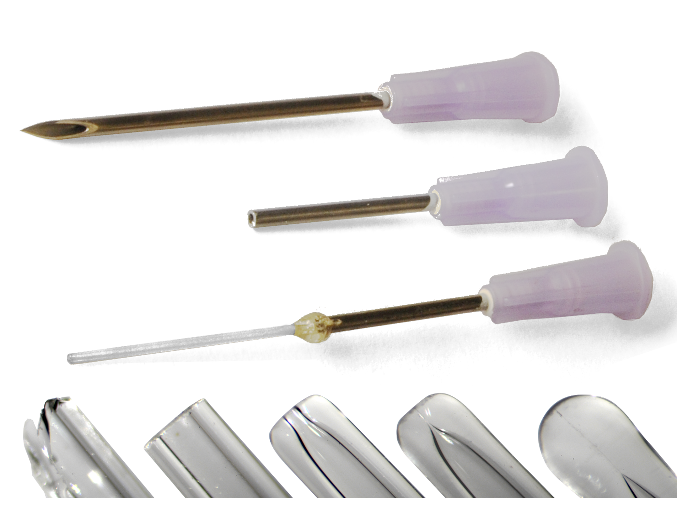
\includegraphics[width=0.3\textwidth]{needlescombo.eps}
\caption{Above: assembly of nozzle from
low-gauge hypodermic syringe (Luer fitting) and capillary. Below: nozzle tip
fabrication, capillary from left to right: broken, sanded, heated in a flame (I.D.
$200\,\mu$m), heated for longer (I.D. $25\,\mu$m, could be sanded down by about
$200\,\mu$m), overheated (I.D. $0\,\mu$m). \label{fig:needles}}
\end{figure}

\paragraph*{Ease of construction and installation.} Unlike loudspeakers, hard
drives have a flat base plate which can be drilled into, allowing for easy
installation on any experiment jig. Save for a drill and a saw, no machining
tools are needed for the construction of the droplet generator.

\paragraph*{High amplitudes without noise.}
Like piezoelectric elements, vibrating actuator arms are very quiet, enabling
use at frequencies and amplitudes that far exceed responsible levels on
a speaker.  In our experiments, the actuator responded to frequencies throughout
our hearing range---i.e., up to $17\,$kHz---and likely well beyond, though we
have not tested the full response range.

As an added advantage over other designs, no amplification is needed. Below
$100\,$Hz, amplitudes on the order of $0.5\,$cm are easily achieved (albeit they
are of course not needed for droplet production) when a peak-to-peak voltage of
$2-4\,$V is applied. The amplitude scales down with the inverse of the frequency,
however, such that they are much smaller at typical operating frequencies
($0.5-10\,$kHz). Nevertheless, the voltages required are well within the ability
of any standard laboratory function generator; they can likely even be produced by many
consumer-level computer sound cards.

\section{Operating principle}
Magnetic hard drives store data as sub-micron-sized patterns of 
oppositely magnetized dots on disks called \emph{platters}. The read-write head
is mounted at the tip of an arm that pivots across the platter surface while the
platter spins. This setup allows the head to access the entire platter surface.

FIG.~\ref{fig:designschematic} illustrates schematically the design of a typical
rotary actuator arm assembly. The flat voice coil mounted on the surface is responsible
for the arm's side-to-side movement: as it is positioned under a permanent
magnet, the coil creates a sideward force (\emph{Lorenz} or \emph{Laplace}
force) when a current flows through its wires. The force is aligned with the
cross product of the current direction and the magnetic field lines. By stopping
or reversing the current, the arm's motion is likewise stopped or reversed. An
applied sinusoid signal can thus be used to make the arm oscillate laterally at
the desired frequency.

%Since a typical hard drive's platter spins at up to $7200\,$RPM,
%actuator arms must be able to move with extreme speed and precision. They are
%thus engineered to be very light yet stiff. These characteristics make a
%magnetic hard drive's actuator arm an ideal supplier of in-plane vibrations.
%Indeed, hard drive actuators are remarkable not for their operating principle
%but for their low cost; it is only the economics of mass manufacturing that has
%in recent years enabled these high-speed, lightweight precision mechanisms to
%become so widely available.

\begin{figure}
\centering
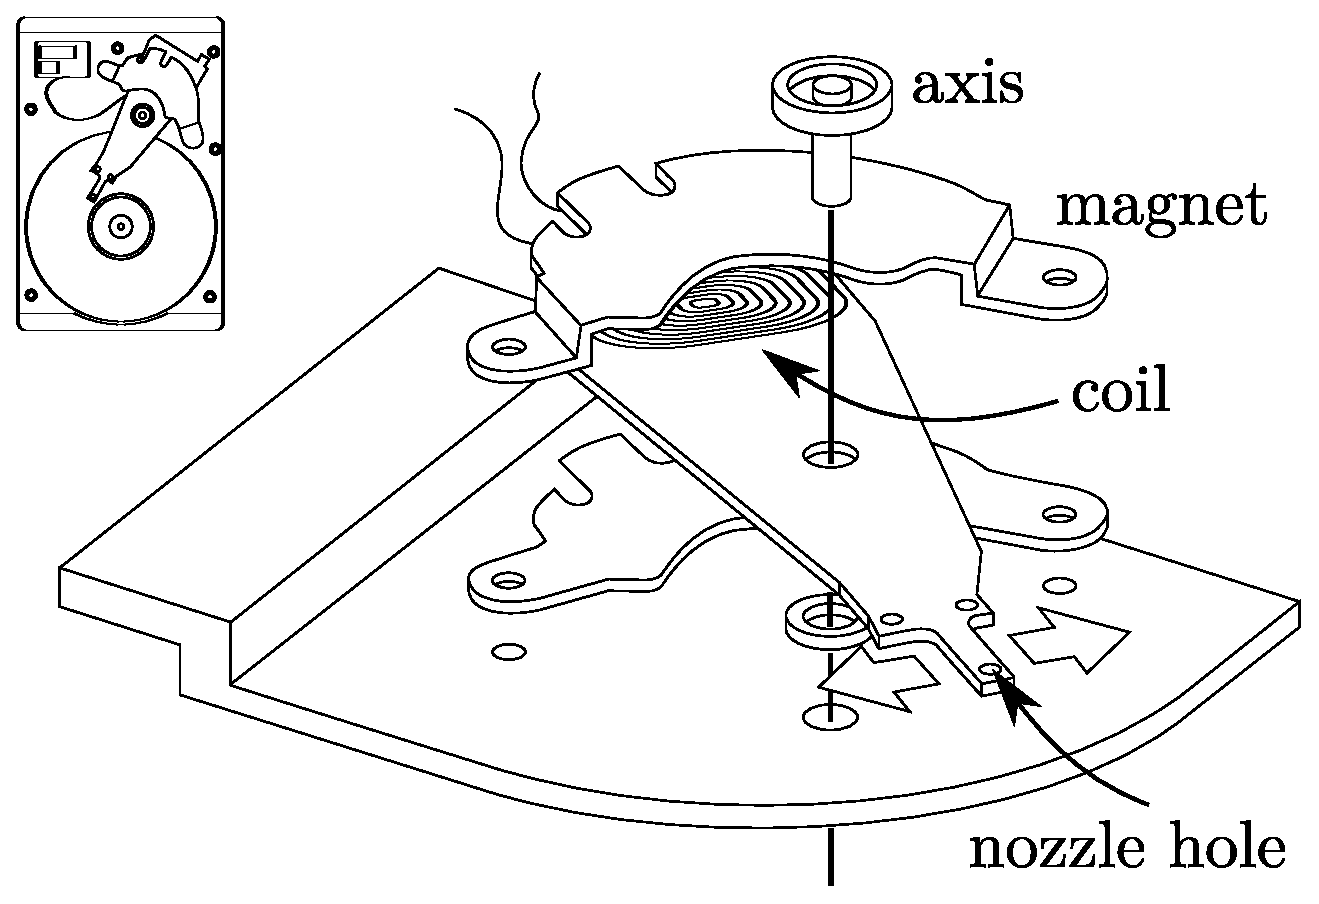
\includegraphics[width=0.3\textwidth]{dge.eps}
\caption{Top view of a hard drive and exploded view of the cut-out base
plate, actuator arm, axis, and magnet assembly. \label{fig:designschematic}}
\end{figure}
\begin{figure}
\centering
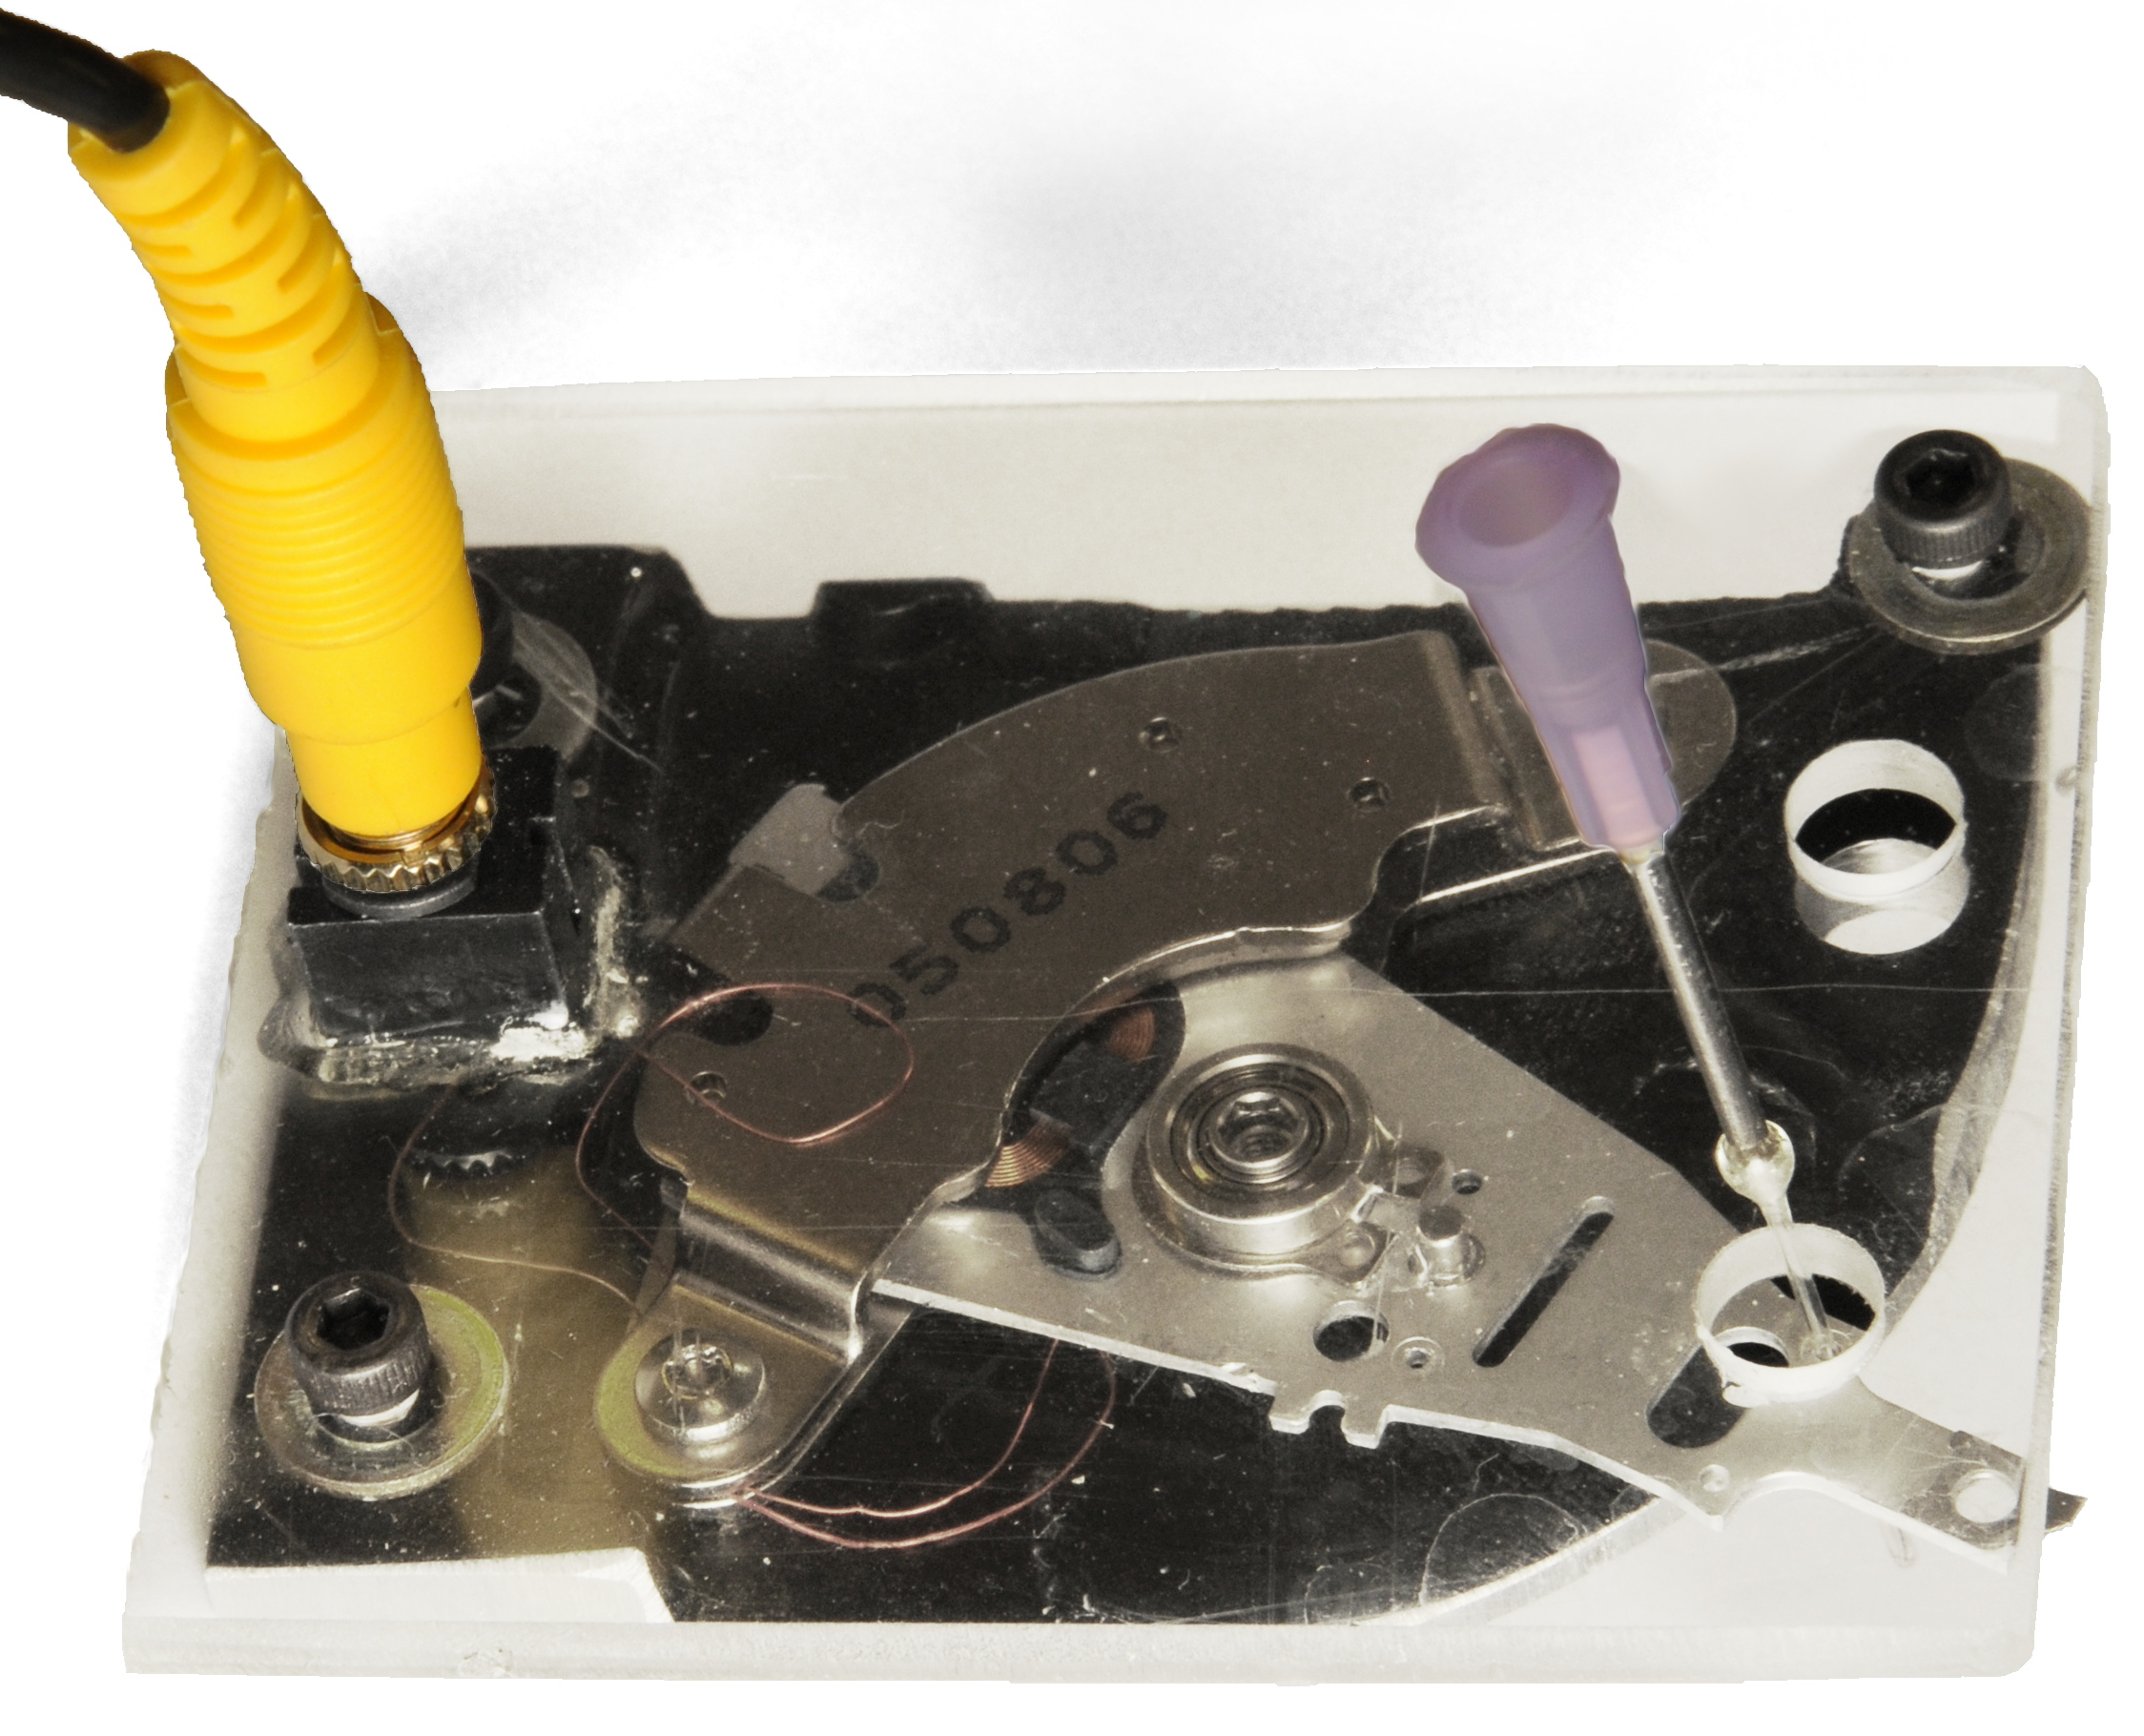
\includegraphics[width=0.35\textwidth]{designpicture.eps}
\caption{A fully assembled droplet generator from a single-platter drive. Nozzle is shown as inserted
through one of the holes in the actuator arm. \label{fig:photo}}
\end{figure}
\begin{figure}
\centering
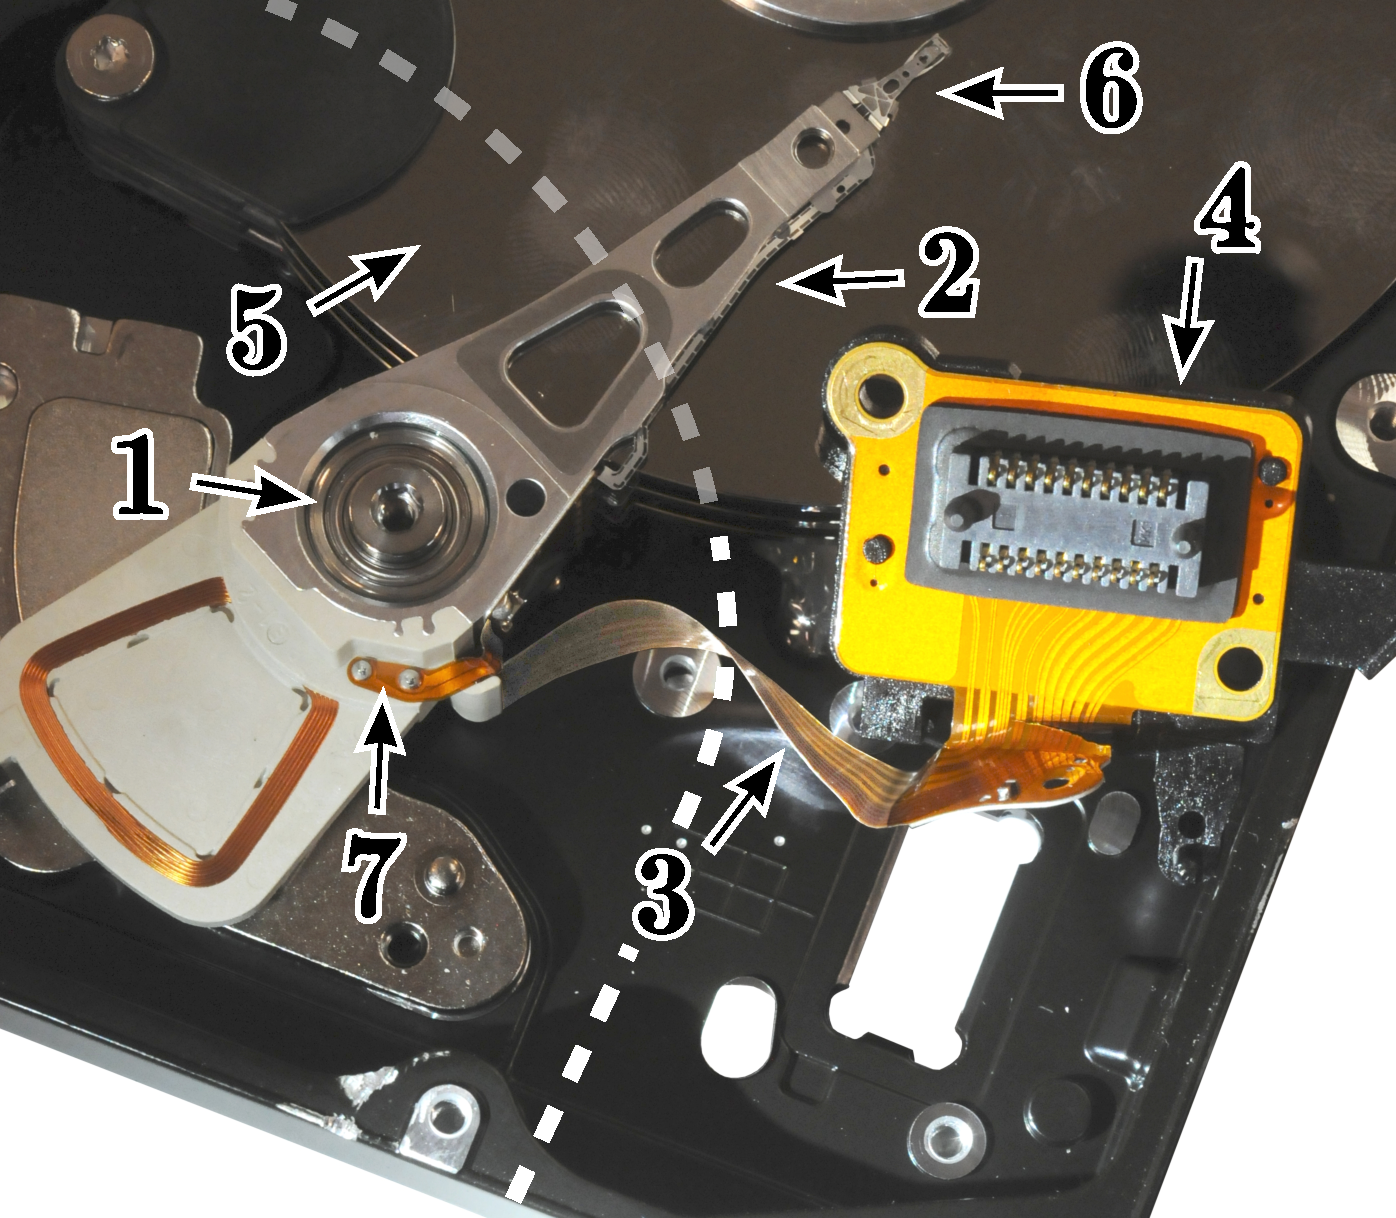
\includegraphics[width=0.35\textwidth]{numbers.eps}
\caption{A multi-platter hard drive after removing cover and detaching circuit board (4). Top
        magnet is removed. Base plate can be cut along dashed line. \label{fig:numbers}}
\end{figure}


\section{Construction}
If possible, forgo multi-platter drives, as they are more cumbersome to disassemble and have
bulky, complex actuator assemblies. The device shown in FIG. \ref{fig:photo}
is based on a single-platter drive.

\paragraph{Dismantle and cut.} After removing the hard drive cover, remove
the top magnet, arm axis (1 in FIG. \ref{fig:numbers}), arm (2), ribbon wires (3), circuit boards (4), and
platters (5) such that only the base plate remains. Now the corner of the base plate holding
the actuator arm assembly can be cut out (dashed line) to yield a shape as shown in FIG.
\ref{fig:designschematic}. A band saw, jigsaw or powered hacksaw will be very
useful, although not necessary. The goal is to allow the tip of the arm to
protrude over the edge. After cutting, reinstall the arm, axis, and top magnet.

\paragraph{Expose coil leads.} Next, remove the read/write head (6) and all
wiring leading to it, along with any connected I/O and servo circuitry (4). Be
careful, however, not to tear off the two strands powering the voice coil, which
are often integrated in the same ribbon cable (3). If you wish to remove the
latter, ensure that exposed terminals (7) remain onto which you can solder new leads.

\paragraph{Add protective cover.} We recommend bolting on a cover plate, such
as a small sheet of transparent plastic, to protect the protruding arm from
accidental bending. Drill a hole through the cover to allow the nozzle to be
threaded through the arm. A severable
connection from coil to function generator is preferable to a direct wire, if
only because the voice coil leads are delicate and easily torn off. To this end, we epoxied
an audio jack into the cover plate (see FIG. \ref{fig:photo}) and soldered the voice coil leads to it from the
bottom.

\section{Operation}
To use the droplet generator, simply insert a nozzle through a small hole at the
tip of the actuator arm---typically at least one hole will already be present
where the read/write head was installed---and connect the voice coil leads to the output terminal of a function
generator set to an initial peak-to-peak voltage of $1\,$V and a sinusoid frequency of
about $50\,$Hz, which should cause weak but perceptible oscillations.

Interchangeable nozzles made from needles with Luer fittings, as in FIG.~\ref{fig:needles}, are
convenient and can be held in place by a male adapter clamped into a lab stand.

%We used existing nozzles manufactured by hand from hypodermic needle stubs and
%heated glass capillaries (FIG.~\ref{fig:needles}). We make no claim that this is
%the best approach to take, but we note that the interchangeability of nozzles
%with Luer fittings has proved very convenient in our application. How the nozzle
%can be held in place falls beyond the scope of this article; while we used an
%existing setup made from machined aluminum, a small lab stand and clamp should
%suffice to hold the male Luer fitting connecting the feed tube to the nozzle.

The nozzle must be supplied by an accurately calibrated syringe pump. It is
convenient to integrate a large liquid reservoir (or tap water hose) via a
T-valve between the between pump and nozzle to permit quick topping up of the
syringe. In such a setup ensure that the reservoir valve is shut closed before operation,
since pressure fluctuations at the nozzle are the most common culprit for
unstable jet breakup conditions.

As with other vibrating orifice droplet generators, it is crucial that stable
conditions are established before any experiments can begin. First, confirm that
the liquid is ejected in a single jet. Multiple jets can be due to a clogged
orifice (a mixture of distilled water and CLR$\circledR$, drawn back through a
syringe, is an excellent remedy). Satellite droplets can also form secondary
jets, in which case the oscillation frequency must be adjusted or the amplitude
reduced. Satellite formation is easily detected by using a gentle air flow to
deflect the jet---if the droplets are truly monodisperse, they will all deflect
at the same angle.\cite{Strom69}


Note also that the orifice diameter $D_o$ dictates the range of viable
frequencies $f$ as 
\begin{equation}
    3.5 \lesssim \frac{Q}{\pi f \left(\frac{D_o}{2}\right)^2}
\lesssim 7,
\end{equation}
where $Q$ is the flow rate.\cite{Savart33, Rayleigh79} In
practice, $D_o$ need not be
precisely determined; it is easy to find appropriate settings for $Q$
and $f$ by viewing the jet against a strobe light, adjusting flow rate for a breakup
length on the order of $10 D_o$ (empirically for water), then tuning the frequency
until droplets appear evenly spaced and spherical. It can be helpful to mount a
magnifying lens in front of the orifice, as the adjustment procedure can become
tedious when the droplets are very small.

Under stable conditions, every oscillation of the nozzle will produce one droplet
downstream,\cite{Rayleigh79} such that the droplet diameter will be 
\begin{equation}
        D_d = \sqrt[3]{6Q/(\pi f)}.\label{eq:rayl}
\end{equation}
This can be verified photographically, as shown in FIG.~\ref{fig:dropphoto}.

We have successfully used the generator to produce droplets of
$0.1-1\,$mm diameter, but both smaller and larger droplets are feasible.

\begin{figure}[h!]
\centering
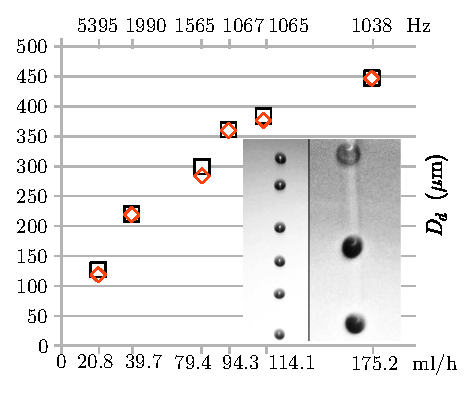
\includegraphics[width=0.26\textwidth]{sizes.eps}
\caption{Some frequency/flow rate conditions under which stable droplets were
        produced ($\square$ as predicted by Eq. \ref{eq:rayl},
        {\Large$\diamond$} as estimated
        from photographs). Photos shown are $D_d = 200\,\mu$m and $D_d = 386\,\mu$m,
        respectively.
       \label{fig:dropphoto}}
\end{figure}
\section{Conclusion}
We have successfully utilized the actuator assembly of a standard magnetic hard
drive as a vibration source in a monodisperse droplet generator. The droplet
generator is not only inexpensive, but remarkably easy to build and painless in
its operation---particularly in comparison to loudspeakers or piezoelectric elements.
These characteristics make hard drive actuators an excellent source of
vibration, likely not only in the context of droplet generation but also for other
purposes in the laboratory or classroom setting.
\bibliography{hdgbibliography}
\end{document}
